\documentclass[12pt,letterpaper]{article}
\usepackage[utf8]{inputenc}
\usepackage[spanish]{babel}
\usepackage{graphicx}
\usepackage[left=2cm,right=2cm,top=2cm,bottom=2cm]{geometry}
\usepackage{graphicx} % figuras
% \usepackage{subfigure} % subfiguras
\usepackage{float} % para usar [H]
\usepackage{amsmath}
%\usepackage{txfonts}
\usepackage{stackrel} 
\usepackage{multirow}
\usepackage{enumerate} % enumerados
\renewcommand{\labelitemi}{$-$}
\renewcommand{\labelitemii}{$\cdot$}
% \author{}
% \title{Caratula}
\begin{document}

% Fancy Header and Footer
% \usepackage{fancyhdr}
% \pagestyle{fancy}
% \cfoot{}
% \rfoot{\thepage}
%

% \usepackage[hidelinks]{hyperref} % CREA HYPERVINCULOS EN INDICE

% \author{}
\title{Caratula}

\begin{titlepage}
\begin{center}
\large{UNIVERSIDAD PRIVADA DE TACNA}\\
\vspace*{-0.025in}
\begin{figure}[htb]
\begin{center}

\includegraphics[width=4cm]{./Imagenes/logo}
\end{center}
\end{figure}
\vspace*{0.15in}
INGENIERIA DE SISTEMAS  \\

\vspace*{0.5in}
\begin{large}
TEMA:\\
\end{large}

\vspace*{0.1in}
\begin{Large}
\textbf{Patrones de diseño arquitecturales y estructurales } \\
\end{Large}

\vspace*{0.3in}
\begin{Large}
\textbf{CURSO:} \\
\end{Large}

\vspace*{0.1in}
\begin{large}
BASE DE DATOS II\\
\end{large}

\vspace*{0.3in}
\begin{Large}
\textbf{DOCENTE(ING):} \\
\end{Large}

\vspace*{0.1in}
\begin{large}
 Patrick Jose Cuadros Quiroga\\
\end{large}

\vspace*{0.2in}
\vspace*{0.1in}
\begin{large}
Integrantes: \\
\begin{flushleft}

Andree Ludwed VELASCO SUCAPUCA	\hfill	(?) \\
Yofer Nain CATARI CABRERA		\hfill	(2017059289) \\
Marko Antonio RIVAS RIOS          	\hfill	(2016055461) \\
Jorge Luis MAMANI MAQUERA    	\hfill	(2016055236) \\
Jesus ESCALANTE ALANOCA   	\hfill	(2015050641) \\
Adnner Sleyder ESPERILLA RUIZ		\hfill	(2015050543) \\
\end{flushleft}
\end{large}
\end{center}

\end{titlepage}


\tableofcontents % INDICE
\thispagestyle{empty} % INDICE SIN NUMERO
\newpage
\setcounter{page}{1} % REINICIAR CONTADOR DE PAGINAS DESPUES DEL INDICE

\section{Patrones de Diseño Composite} 

\textbf{}\\
El patrón de diseño Composite nos sirve para construir estructuras complejas partiendo de otras estructuras mucho más simples, dicho de otra manera, podemos crear estructuras compuestas las cuales están conformadas por otras estructuras más pequeñas.
Para comprender mejor como funciona este patrón imaginemos una casa de ladrillos, las casas como tal no están hecha de una pieza, si observamos las paredes estas esta echas de pequeñas piezas llamadas ladrillos, entonces, el conjunto de estos ladrillos crea paredes, y un conjunto de paredes crean una casa. este ejemplo puede ser aplicado al patrón Composite, y no digo que vayamos a crear una casa con este patrón, sino más bien nos da una idea de cómo trabaja para poder utilizarlo con otros ejemplos.

\begin{flushleft}

\begin{center}
	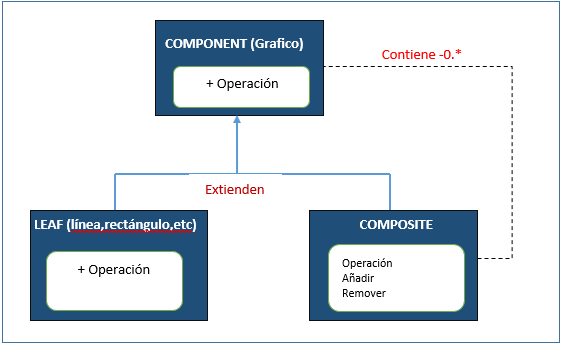
\includegraphics[width=10cm]{./Imagenes/composite1} 
	\end{center}
\begin{itemize}
\textbf{Uso}

El patrón Composite sirve para construir objetos complejos a partir de otros más simples y similares entre sí, gracias a la composición recursiva y a una estructura en forma de árbol.  Esto simplifica el tratamiento de los objetos creados, ya que al poseer todos ellos una interfaz común, se tratan todos de la misma manera. Dependiendo de la implementación, pueden aplicarse procedimientos al total o una de las partes de la estructura compuesta (todo o parte) como si de un nodo final se tratara, aunque dicha parte esté compuesta a su vez de muchas otras.

\textbf{}\\
\textbf{Aplicación}


Usar el patrón COMPOSITE cuando:


  \item Se quiere representar jerarquías de objetos todo-parte.
  \item Se quiere ser capaz de ignorar la diferencia entre objetos individuales y composiciones de objetos.  Los clientes tratarán a todos los objetos de la estructura compuesta uniformemente.

\end{itemize} 

\textbf{}\\
\textbf{}\\
\textbf{}\\
\textbf{}\\
\textbf{}\\
\textbf{}\\
\textbf{Estructura}

\textbf{}\\ 
\textbf{}\\ 

\begin{center}
	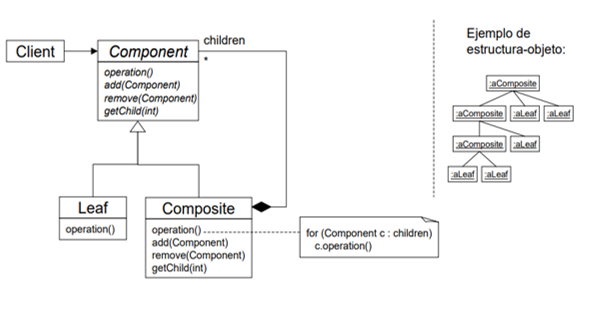
\includegraphics[width=10cm]{./Imagenes/composite2} 
	\end{center}

\textbf{Participantes}

El patrón Composite requiere mínimo de tres componentes para poder existir los cuales son Componente, Leaf o Rama y Composite.

\begin{enumerate}[a)]
        \item \textbf{ Component (Grafico)}
Generalmente es una interface o clase abstracta la cual tiene las operaciones mínimas que serán utilizadas, este componente deberá ser extendido por los otros dos componentes Leaf y Composite. En nuestro ejemplo esto podría representar de forma abstracta un ladrillo o toda la casa (Mas adelante comprenderemos porque)

        \item \textbf{ Leaf o Rama (Línea, Rectángulo, Texto)}
El leaf u hoja representa la parte más simple o pequeña de toda la estructura y este extiende o hereda de Component. En nuestro ejemplo, este representaría un ladrillo de nuestra casa.

	\item \textbf{Composite (Dibujo)}
Aquí es donde está la magia de este patrón, ya que el composite es una estructura conformada por otros Composite y Leaf, los Composite tiene los métodos add  (añadir) y remove (remover) los cuales nos permiten agregar objetos de tipo Component, Sin embargo, el Componente es por lo general un Interface o Clase abstracta  por lo que se puede agregar objetos de tipo Composite o Leaf.   Desde el punto de vista del ejemplo de la casa el Composite podría representar un conjunto de ladrillos o la casa completa, Esto desde luego sería agregando varias Ladrillo(Leaf) al Composite para crear una Pared.

	\item \textbf{ Client}
Es la entidad que hará uso del objeto compuesto.
    \end{enumerate}

\textbf{}\\ 
\textbf{}\\ 
\textbf{}\\ 
\textbf{}\\ 
\textbf{}\\ 
\textbf{}\\ 
\textbf{}\\ 
\textbf{}\\ 
\textbf{}\\ 
\textbf{EJEMPLO DE ESTUDIO DEL PATRON COMPOSITE}
Imaginemos un sistema de puntos de venta, en el cual se le pueden vender al cliente una serie de productos, estos productos pueden ser productos simples (Leaf) o paquetes (Composite).  El sistema permitirá crear “Ordenes de Ventas”, las cuales están compuestas por 1 o muchos productos.

\begin{center}
	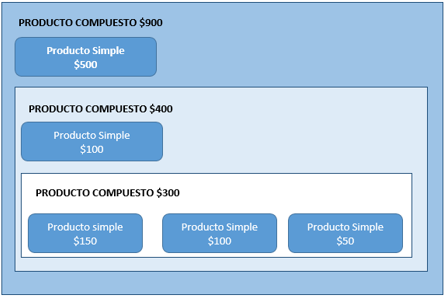
\includegraphics[width=10cm]{./Imagenes/composite3} 
	\end{center}

En la imagen se muestra de forma gráfica cómo está compuesto un paquete.  Los paquetes están creados a partir de un conjunto de productos simples y otros paquetes por lo que el precio de un paquete está calculado por el precio de sus hijos de forma recursiva.  Muestra la estructura de una forma conceptual, sin embargo, la estructura es un poco más compleja, ya que está formado por una estructura de dato llamado “Arbol”

\begin{center}
	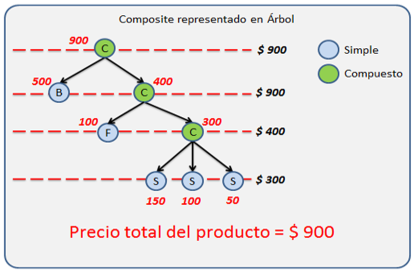
\includegraphics[width=10cm]{./Imagenes/composite4} 
	\end{center}

Esta imagen muestra un solo paquete, está formado de otros productos, simples y compuestos, un compuesto sería otro paquete, el cual tiene dentro más productos simples y como se vio en la figura anterior, el precio de un paquete es calculado por el precio de todos los hijos de forma recursiva.

\textbf{}\\ 
\textbf{}\\
\textbf{}\\
\textbf{}\\
\textbf{}\\
\textbf{}\\

\textbf{CONCLUSION}

\begin{itemize}
\item Define jerarquías de clases hechas de objetos simples y compuestos. 
\item Si el código cliente espera un objeto simple, puede recibir también uno compuesto 
\item Puede hacer el diseño demasiado general. Es complicado restringir el tipo de componentes de un composite.
\item Un paquete es producto compuesto de varios productos simples y otros paquetes.
\item Simplifica el cliente.  Los paquetes y productos simples deberán ser tratados de la misma forma, por lo que deberán tener un padre en común.
\item El precio de un paquete es la suma de todos los productos simples que contenga.
\item El sistema deberá mostrar el total de la Orden y los productos que contiene.
\item Facilita la incorporación de nuevos tipos de componentes


\end{itemize} 





\end{flushleft}
\section{Patrón de Diseño Proxy} 
\textbf {1.    ¿Qué es el Patrón Proxy?}
\textbf{}\\
El patrón Proxy proporciona un objeto intermediario entre el cliente y el objeto a utilizar, que permite configurar ciertas características (como el acceso) sin necesidad de modificar la clase original.
\begin{flushleft}
\begin{center}
	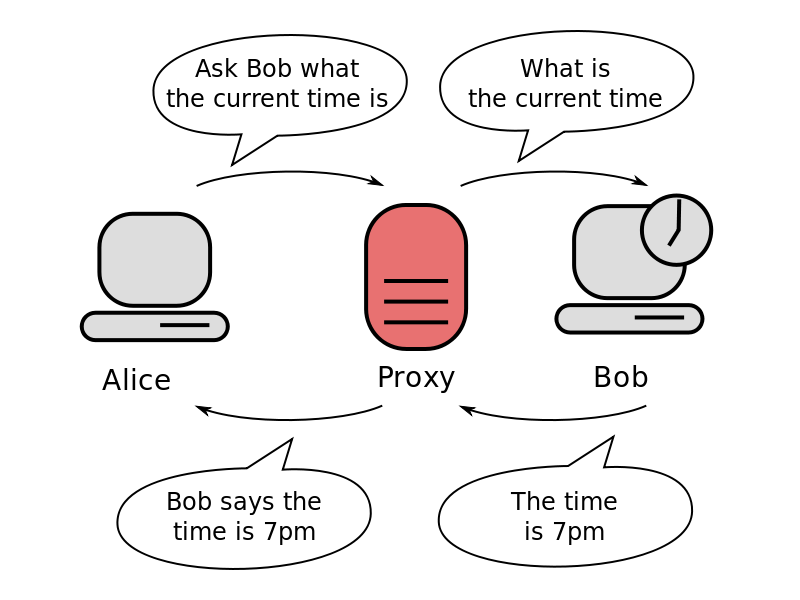
\includegraphics[width=10cm]{./Imagenes/proxy1} 
	\end{center}
\begin{itemize}
	\item Por ejemplo:
Si tenemos muchos objetos imagen en un documento, se tardaría mucho tiempo en abrir el documento al cargar las imágenes de disco. Para evitarlo podemos sustituir los objetos imagen por objetos proxyImagen, con el mismo interfaz, pero que solamente cargan la imagen cuando se va a visualizar.

\textbf {2.	Tipos de Patrón Proxy}
\textbf{}\\
Existen varios tipos de Proxy que realizan distintos tipos de tareas: Proxy Remoto, Proxy Virtual, Proxy de Protección.

\item	\textbf {Proxy Remoto:} Se comporta como un representante local de un objeto, al realizar esto lo que hace es abstraer toda la “conversación” entre “dos” y de esta forma la comunicación entre el cliente y el objeto remoto es más fácil gastando menos recursos.
\item	\textbf {Proxy Virtual:} Lo que hace el proxy virtual es instanciar objetos cuyo costo computacional es muy elevado.

 \item	\textbf {Proxy Protección:} Lo único que hace es establecer el control de acceso a un objeto dependiendo de los permisos o reglas de autorización.


\textbf {3.	Estructura del Patrón Proxy}
\textbf{}\\

\textbf {3.1.	Clasificación}
\textbf{}\\
\item	\textbf {Patrón estructural:} Ya que define la forma en cómo se organizan los objetos y las dependencias que tiene entre ellos.
\textbf{}\\
\textbf {3.2.	Aplicaciones}
\textbf{}\\

\item Útil cuando se desea retrasar la instanciación de un objeto hasta que sea necesario usarlo (optimiza operaciones costosas: invocar imagen). 
\item Proporciona un representante local de un objeto situado en otro espacio de direcciones (Proxy remoto o “Embajador”). 
\item Uso en sistemas concurrentes, mediante cerrojo, controlando el acceso al objeto original. 
\item Puede utilizarse como un sustituto de un simple puntero, que lleva a cabo operaciones adicionales cuando se accede a un objeto (contar el número de referencias a un objeto real).

\textbf{}\\
\textbf {3.3.	Consecuencias}
\textbf{}\\
\item Un proxy puede ocultar el hecho de que un objeto reside en un espacio de direcciones diferente (proxy remoto). 
\item Puede llevar a cabo optimizaciones tales como crear un objeto por encargo (invocar imagen). 
\item Permiten realizar tareas de mantenimiento adicionales cuando se accede a un objeto (Proxy de protección y de referencias inteligentes).
\item Se introduce un nivel de indirección al acceder al objeto.
\item Se consigue una administración transparente de los servicios del objeto real. 
\begin{center}
\textbf {Representación UML}
\end{center}
\begin{center}

	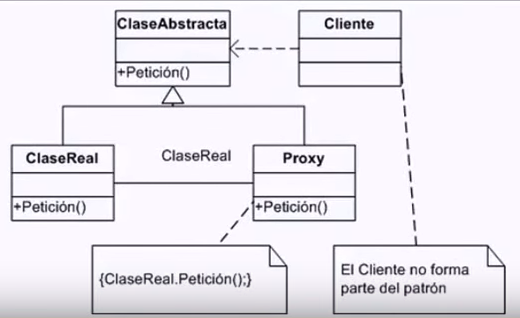
\includegraphics[width=10cm]{./Imagenes/proxy2} 
	\end{center}

\textbf{}\\
\textbf {3.4.	Participantes}
\textbf{}\\


\item	\textbf {Sujeto:} Define la interfaz común para el RealSubject y el Proxy, de modo que pueda usarse un Proxy en cualquier sitio en el que se espere un RealSubject.
\textbf{}\\
\item	\textbf {RealSubject:} Define el objeto real representado.
\textbf{}\\
\item	\textbf {Proxy:}
\textbf{}\\
Mantiene una referencia que permite al Proxy acceder al objeto real. 
Proporciona una interfaz idéntica a la del sujeto, de manera que un Proxy pueda ser sustituido por el sujeto real. 
Controla el acceso al sujeto real, y puede ser responsable de su creación y borrado.
\textbf{}\\
\textbf{}\\

\textbf {4.	Ejemplos UML}

\item	\textbf {Diagrama UML}
\textbf{}\\
Un ejemplo típico de aplicación del patrón proxy es el de un editor de documentos. El editor podrá incluir imágenes y dibujos complejos, y se plantea el problema de recuperar todos estos costosos objetos cada vez que se abre el documento. La aplicación del patrón proxy soluciona el problema definiendo un "representante", que ocupe su lugar, hasta que sea necesario cargarlos.
\begin{center}

	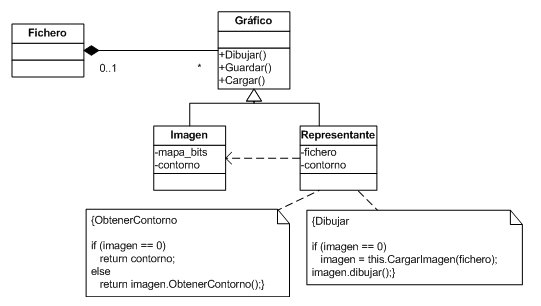
\includegraphics[width=10cm]{./Imagenes/proxy3} 
	\end{center}



\textbf {5.	Ejemplos de Implementación sin Proxy y/o con Proxy}

\item	\textbf {Sin Proxy}

\begin{center}

	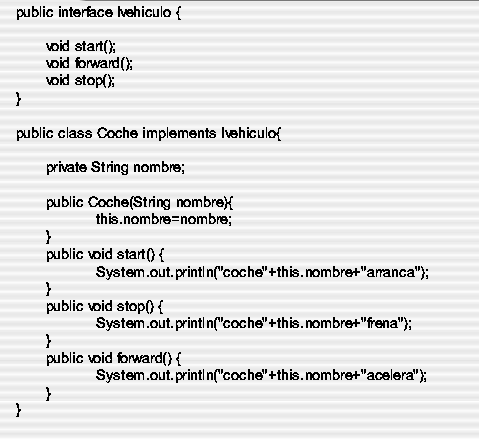
\includegraphics[width=10cm]{./Imagenes/proxy4} 
	\end{center}
\begin{center}
\textbf{}\\
	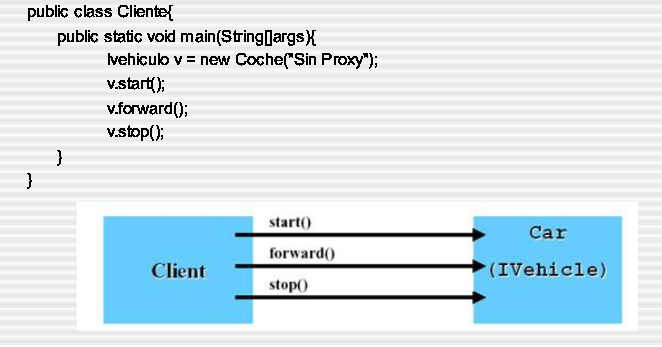
\includegraphics[width=10cm]{./Imagenes/proxy5} 
	\end{center}


\item	\textbf {Con Proxy}

\begin{center}

	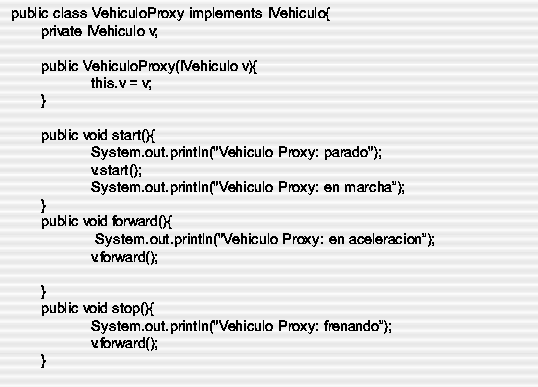
\includegraphics[width=10cm]{./Imagenes/proxy6} 
	\end{center}
\begin{center}
\textbf{}\\
	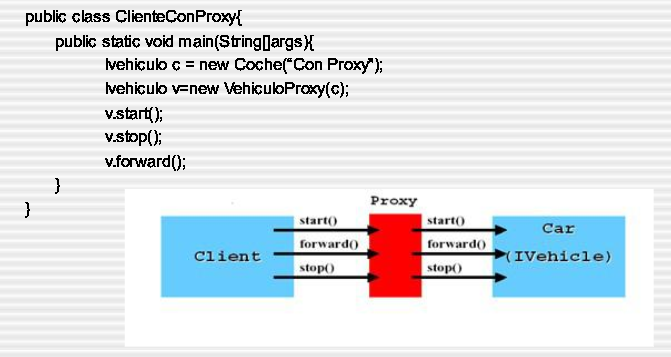
\includegraphics[width=10cm]{./Imagenes/proxy7} 
	\end{center}



\textbf {6.	Conclusiones}

\item	\textbf {No Proxy:} El cliente interactúa directamente con los métodos definidos en la interface 

\item	\textbf {Proxy:} Se encuentra entre la interfaz y la implementación e intercepta las llamadas a los métodos. La intención del Proxy es controlar el acceso al objeto deseado, además de mejorar la funcionalidad del mismo 


	

\end{itemize} 


\end{flushleft}
\section{Patrones de Diseño Decorator} 

\textbf{}\\
“Añadir responsabilidades a un objeto de forma dinámica. Los decoradores proporcionan una alternativa flexible a la herencia para extender funcionalidad.”

\begin{center}
	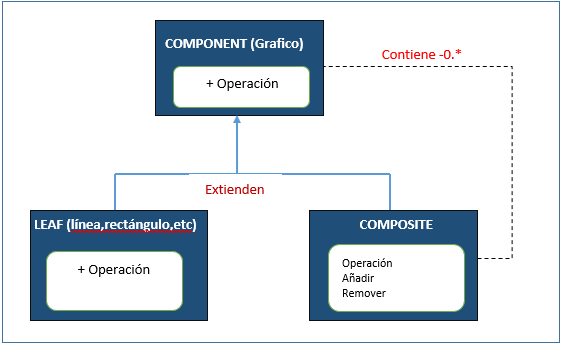
\includegraphics[width=10cm]{./Imagenes/composite1} 
	\end{center}


\begin{flushleft}

El siguiente de los patrones estructurales que veremos sera el patrón Decorator o decorador. Su filosofía consiste en añadir responsabilidades de forma dinámica con el principal objetivo de evitar la conocida como “explosión de clases”, es decir, la generación de un número elevado de subclases a partir de una superclase común.
Como podemos observar en el gráfico superior, la clase Decorator hereda de la misma clase que el componente que se quiere decorar. Así, cada decorador es capaz de encapsular una instancia de cualquier otro objeto que herede del componente común, bien un componente concreto u otro decorador. Este comportamiento recuerda al que vimos previamente en el patrón Adapter, con la diferencia de que la clase Decorator, a diferencia de la clase Adapter, no transforma una interfaz, sino que añade cierta funcionalidad.
La encapsulación puede ser iterativa, de modo que un componente concreto puede ser encapsulado por un decorador, que a su vez puede ser encapsulado por otro decorador… y así sucesivamente, añadiendo nueva funcionalidad en cada uno de los pasos. Resumiendo: el patrón Decoratorsustituye la herencia por un proceso iterativo de composición.


\begin{center}
	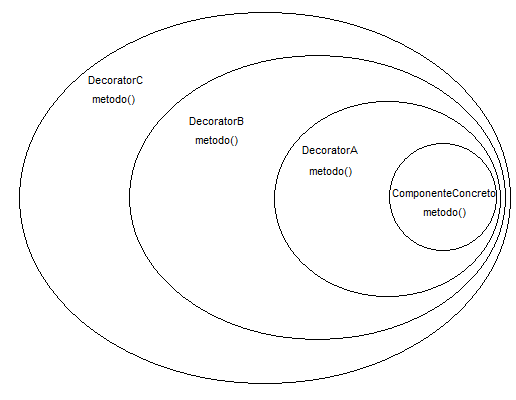
\includegraphics[width=10cm]{./Imagenes/decorator2} 
	\end{center}

El objeto con el que el objeto cliente interactuará será aquel que se encuentre en la capa más externa (en este caso, DecoratorC), que se encargará de acceder a los objetos contenidos e invocar su funcionalidad, que será devuelta a las capas exteriores.
Para comenzar, por tanto, debemos tener claros los siguientes conceptos sobre este patrón:

\begin{itemize}



  \item Un decorador hereda de la misma clase que los objetos que tendrá que decorar.
  \item Es posible utilizar más de un decorador para encapsular un mismo objeto.
\item El objeto decorador añade su propia funcionalidad, bien antes, bien después, de delegar el resto del trabajo en el objeto que está decorando.
\item Los objetos pueden decorarse en cualquier momento, por lo que es posible decorar objetos de forma dinámica en tiempo de ejecución.

\end{itemize} 

\textbf{}\\
La razón por la que la clase Decorator hereda de la misma clase que el objeto que tendrá que decorar no es la de añadir funcionalidad, sino la de asegurarse de que ambos comparten el mismo tipo y puedan intercambiarse: un decorador podrá sustituir a un objeto decorado, basándonos en el principio SOLID del Principio de sustitución de Liskov.


\textbf{Declarando las clases funcionales}

Como viene siendo habitual, ilustraremos nuestro patrón haciendo uso de vehículos. En este caso, utilizaremos una case abstracta, llamada Vehiculo, del que heredarán las clases funcionales a las que llamaremos “Berlina” y “Monovolumen”, y los decoradores, que se limitarán a añadir funcionalidad a estas clases funcionales. Los decoradores que diseñaremos serán “Diesel”, “Gasolina”, “Inyeccion”, “CommonRail” y “Turbo”.

Estos decoradores se caracterizarán por:

\begin{itemize}



  \item Disponer de una referencia a un vehículo que será inyectada en el constructor.
  \item Modificar el funcionamiento original de la clase que decoran, sobrecargando los métodos y llamando a los métodos de las clases encapsuladas para modificar su información o funcionamiento.


\end{itemize} 

\textbf{}\\ 
Comencemos codificando nuestra clase abstracta Vehiculo de la cual heredarán el resto de clases.

\begin{center}
	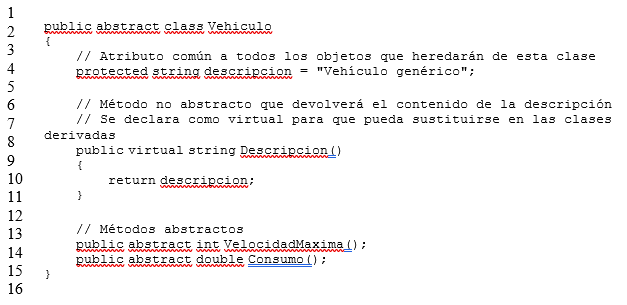
\includegraphics[width=10cm]{./Imagenes/decorator3} 
	\end{center}

Hecho esto, añadiremos nuestras clases funcionales: Monovolumen y Berlina.

\textbf{Monovolumen}
\begin{center}
	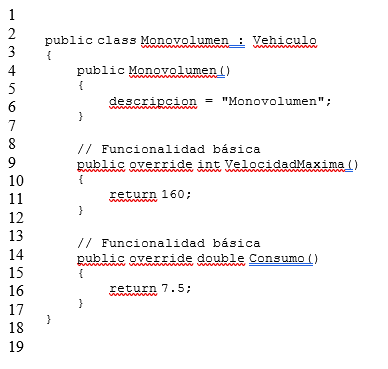
\includegraphics[width=10cm]{./Imagenes/decorator4} 
	\end{center}


\textbf{Berlina}
\begin{center}
	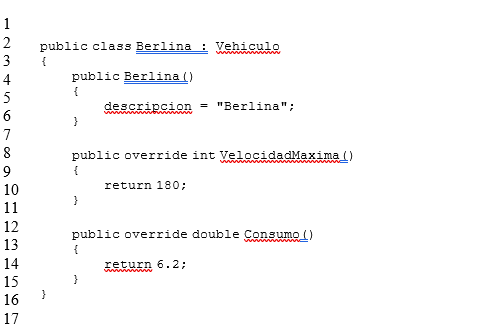
\includegraphics[width=10cm]{./Imagenes/decorator5} 
	\end{center}

Como vemos, ambas clases heredan un atributo común, “descripcion”, y la funcionalidad VelocidadMaxima y Consumo. Asumiremos que un monovolumen posee una velocidad máxima de 160km/h y un consumo de 7,5 litros/100km, mientras que una berlina podrá alcanzar los 180km/h con un consumo de 6,2 litros/100km. Esta funcionalidad será modificada por nuestras clases decoradoras, que podrán aumentar o disminuir estas características.
Con esto habríamos codificado nuestra rama “funcional”. Aún no hay rastro del patrón Decorator, ya que únicamente hemos hecho uso de la herencia de la manera habitual (de hecho, de una forma un tanto escueta).
\begin{center}
	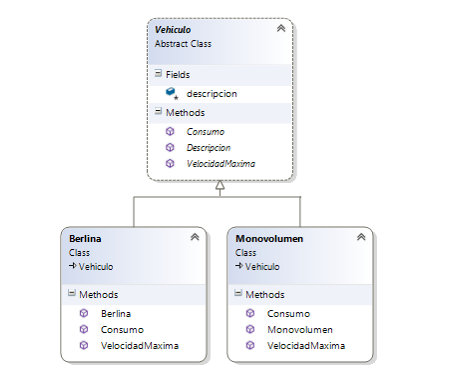
\includegraphics[width=10cm]{./Imagenes/decorator6} 
	\end{center}

\textbf{Creando las clases Decorator}

Es hora, por tanto, de añadir una nueva “rama” a nuestro árbol, añadiendo los decoradores. Comenzaremos por crear una nueva clase abstracta que herede de Vehiculo (para que pueda ocupar su lugar) y de la cual heredarán todos los decoradores.
\begin{center}
	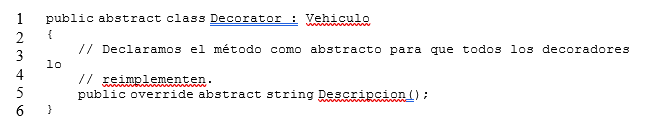
\includegraphics[width=10cm]{./Imagenes/decorator7} 
	\end{center}

A continuación añadiremos los decoradores, que incluirán una referencia a un vehículo y que se construirán mediante la inyección de éste. Por tanto, las características de estos decoradores, además de heredar de Decorator, serán las siguientes:

\begin{itemize}



  \item Contienen una referencia a un Vehiculo, que se insertará en el constructor.
  \item Modifican el funcionamiento de las clases que encapsulan, accediendo a sus atributos y métodos y adaptándolos a la nueva funcionalidad deseada.


\end{itemize} 

Comenzaremos añadiendo un decorador llamado “Gasolina”. La gasolina, al ser más explosiva, proporciona mayor velocidad punta, pero al ser menos energética que el gasoil, también conlleva tener un consumo más elevado. Esta clase tendrá, por tanto, el siguiente aspecto:

\begin{center}
	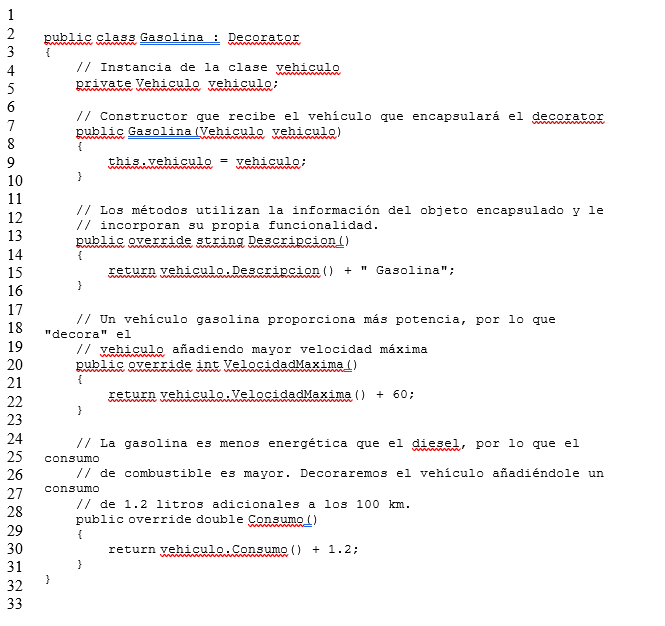
\includegraphics[width=10cm]{./Imagenes/decorator8} 
	\end{center}

Podemos utilizar un razonamiento análogo para un motor diesel, que tendrá el funcionamiento opuesto.
\begin{center}
	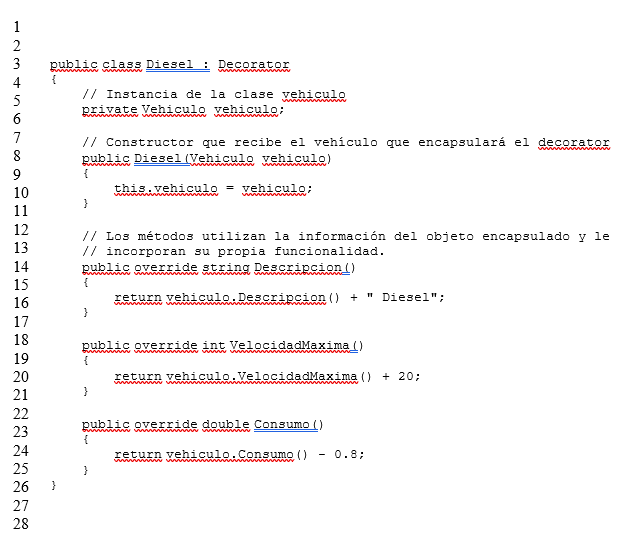
\includegraphics[width=10cm]{./Imagenes/decorator9} 
	\end{center}


¡Ojo! Según nuestro diseño, un vehículo podría ser a la vez diesel y gasolina, ya que ambos heredan de la clase Vehiculo. Las reglas de negocio no deberían permitir que esto fuera así, por lo que deberíamos utilizar reglas adicionales para evitar que ambos decoradores estuviesen presentes en un mismo objeto. No obstante, ignoraremos este hecho en este ejemplo.
A continuación añadiremos nuevos decoradores a nuestro vehículo. Por ejemplo, el turbo.

\begin{center}
	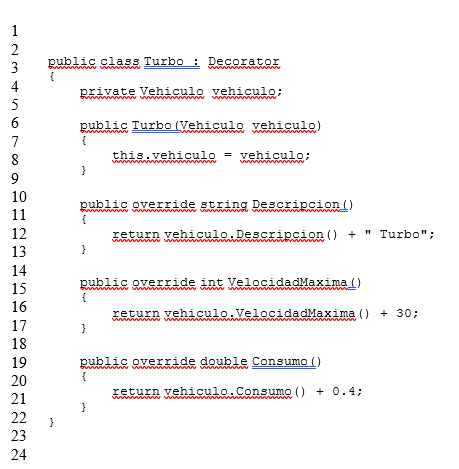
\includegraphics[width=10cm]{./Imagenes/decorator10} 
	\end{center}

Otra posible modificación al vehículo original podría ser la inyección de combustible, que no afectará a la velocidad pero mejorará notablemente el consumo de combustible:
\begin{center}
	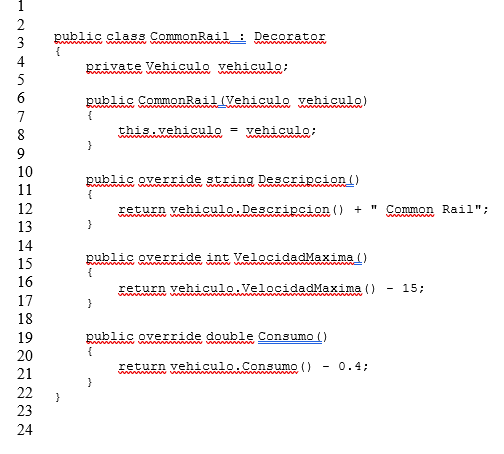
\includegraphics[width=10cm]{./Imagenes/decorator11} 
	\end{center}

Tras nuestra última adquisición, nuestra jerarquía de clases tendrá el siguiente aspecto:

\begin{center}
	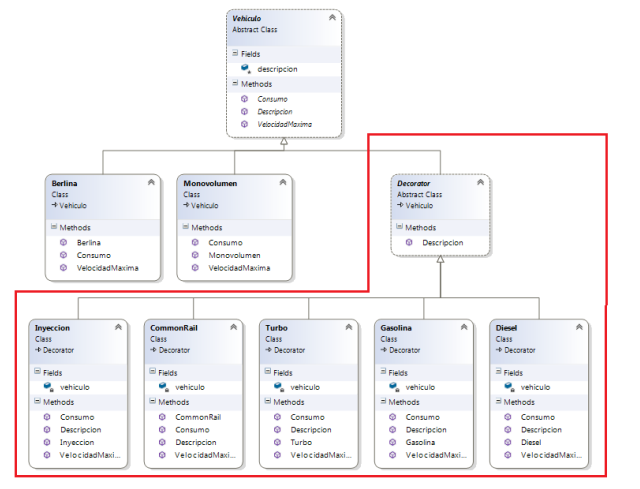
\includegraphics[width=10cm]{./Imagenes/decorator12} 
	\end{center}

Ahora es posible componer, en tiempo de ejecución, un objeto que combine algunas o todas estas características sin necesidad de codificar una clase por cada posible combinación.

\textbf{Utilizando el patrón Decorator}
Es hora de hacer uso del patrón que acabamos de explicar. Comenzaremos creando un vehículo monovolumen y otro vehículo de tipo berlina, mostrando por pantalla sus características:
\begin{center}
	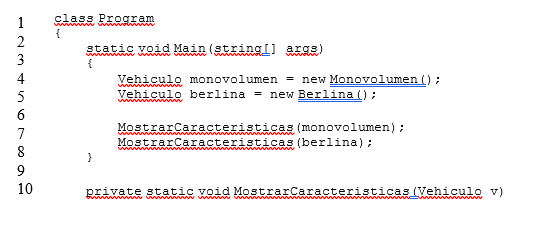
\includegraphics[width=10cm]{./Imagenes/decorator13} 
	\end{center}
\textbf{}\\ 
\begin{center}
	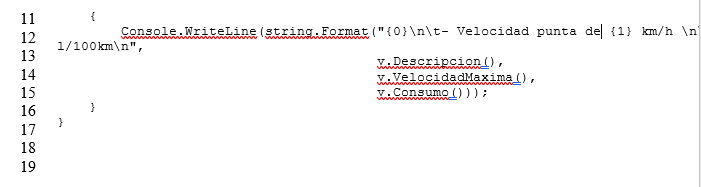
\includegraphics[width=10cm]{./Imagenes/decorator14} 
	\end{center}
\textbf{}\\ 
Nuestro programa nos mostrará el siguiente resultado:
\textbf{}\\ 
\begin{center}
	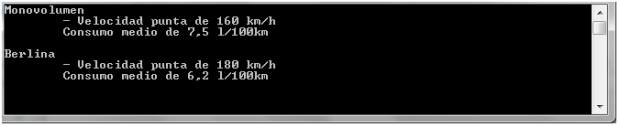
\includegraphics[width=10cm]{./Imagenes/decorator15} 
	\end{center}
\textbf{}\\ 

Como vemos, se nos ofrece una versión “básica” de nuestros objetos, que aún no han sido decorados. Probemos a decorar nuestro monovolumen añadiéndole un motor gasolina:
\textbf{}\\ 
\begin{center}
	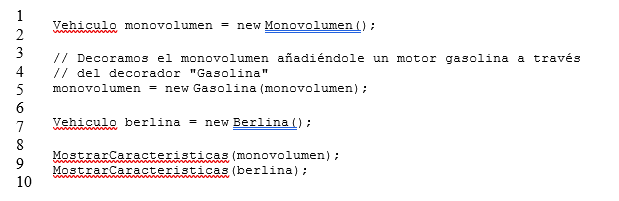
\includegraphics[width=10cm]{./Imagenes/decorator16} 
	\end{center}
\textbf{}\\ 
Esto modificará el comportamiento de nuestro monovolumen, que presentará las siguientes características:
\textbf{}\\ 
\begin{center}
	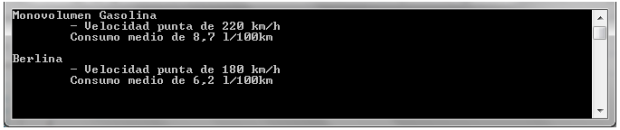
\includegraphics[width=10cm]{./Imagenes/decorator17} 
	\end{center}
\textbf{}\\ 
Se ha modificado, por tanto, su descripción, velocidad punta y consumo medio. Hagamos lo propio con el vehículo de tipo Berlina, al que convertiremos en un vehículo diesel turbo inyección common-rail:
\textbf{}\\ 
\begin{center}
	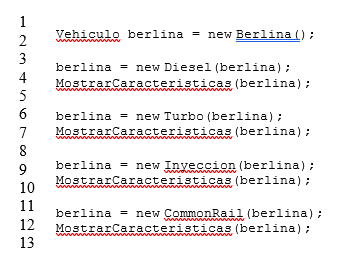
\includegraphics[width=10cm]{./Imagenes/decorator18} 
	\end{center}
\textbf{}\\ 
Como podemos observar, la propia instancia de Vehiculo es pasada como parámetro al constructor, que devuelve la misma instancia decorada con la nueva funcionalidad.
\textbf{}\\ 
\begin{center}
	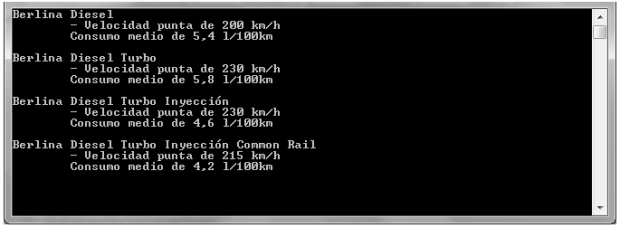
\includegraphics[width=10cm]{./Imagenes/decorator19} 
	\end{center}
\textbf{}\\ 
Así, con una única referencia, hemos conseguido modificar el comportamiento de la instancia en tiempo de ejecución sustituyendo la capacidad de especialización de la herencia por un proceso horizontal de composición.

\textbf{¿Cuándo utilizar este patrón? Ejemplos reales?}
No debemos hacer caso omiso de que la referencia “berlina” ocupará ahora en memoria el quíntuple de lo que originalmente ocupaba, ya que se trata en realidad de una referencia a CommonRail que contiene un objeto Inyeccion que contiene un objeto Turbo que contiene un objeto Diesel que a su vez contiene la instancia Berlina original. Por tanto, conviene estudiar bien el contexto en el que se utilizará este patrón, ya que el ahorro que obtendremos en diseño lo pagaremos en memoria.
\textbf{}\\ 
\begin{center}
	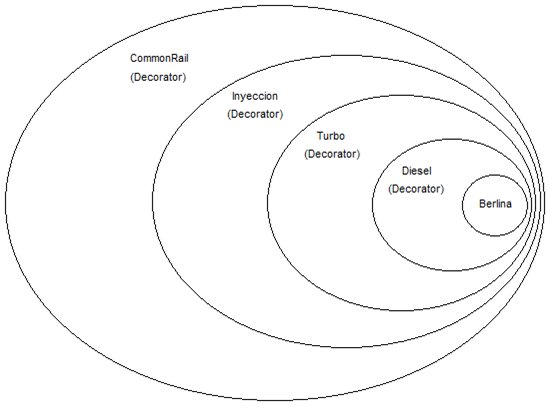
\includegraphics[width=10cm]{./Imagenes/decorator20} 
Un ejemplo claro de este patrón en la API de .NET es la familia de clases Stream. La clase Streames una clase abstracta que expone la funcionalidad básica que será implementada por las clases concretas y decoradas por las clases que componen el patrón.
	\end{center}
\textbf{}\\ 

Algunas de las clases concretas que podemos encontrar en esta familia son las siguientes:


  \item FileStream: representa un flujo (stream) que se encargará de realizar operaciones E/S sobre un fichero físico.

  \item MemoryStream: representa un flujo que realizará operaciones E/S en memoria. Se usa como una proyección temporal en memoria de otro flujo.

  \item 	BufferedStream: representa una sección de un flujo que realizará operaciones E/S en memoria. La diferencia con el anterior es que el MemoryStream representa un flujo completo (por ejemplo, una proyección en memoria de un FileStream), mientras que BufferedStream se usa en conjunción con otros Streams para realizar operaciones de E/S que posteriormente serán leídas o volcadas desde/hacia el flujo original.

Estas clases serían nuestra Berlina y Monovolumen. Pero ¿y los Decorator? Las clases que actúan como decoradores son fácilmente identificables porque reciben un Stream como parámetro a la hora de crear una nueva instancia, a la vez que extienden la funcionalidad del objeto de la clase original.
\textbf{}\\ 
Algunos de los decoradores que podemos encontrar, y que son aplicables a cualquiera de las tres clases anteriores son:

  \item 	CryptoStream: define una secuencia que vincula los flujos de datos a las transformaciones criptográficas.
  \item 	AuthenticatedStream: proporciona métodos para pasar las credenciales a través de una secuencia y solicitar o realizar la autenticación para las aplicaciones de cliente-servidor.
  \item 	GZipStream: proporciona los métodos y propiedades que permiten comprimir y descomprimir secuencias.

\textbf{}\\ 
\textbf{}\\ 
Cada uno de estos Decorator reciben en su constructor un Stream, añadiéndole nuevas funcionalidades y permitiendo que sigan actuando como Stream. Debido al polimorfismo, un CryptoStream que decore un MemoryStream seguirá pudiendo sustituir a cualquier objeto que se pase como parámetro como una referencia a Stream.
\textbf{}\\ 
\begin{center}
	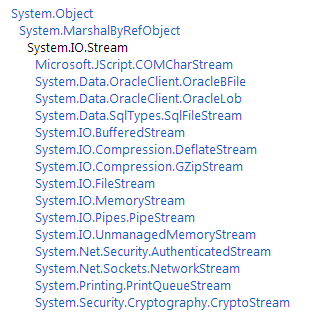
\includegraphics[width=10cm]{./Imagenes/decorator21} 

	\end{center}
\textbf{}\\ 


Podemos ver un ejemplo similar en Java, donde la clase InputStream actuaría como la clase base abstracta, clases como FileInputStream, StringBufferInputStream y ByteArrayInputStream actuarían como clases concretas, FilterInputStream actuaría como la clase abstracta de la que heredan todos los decoradores (clase que no existe en la familia Stream de .NET) y clases como BufferedInputStream, DataInputStream o LineNumberInputStream actuarían como decoradores, recibiendo un objeto de la clase InputStream como parámetro en su constructor.






\end{flushleft}


\end{document}